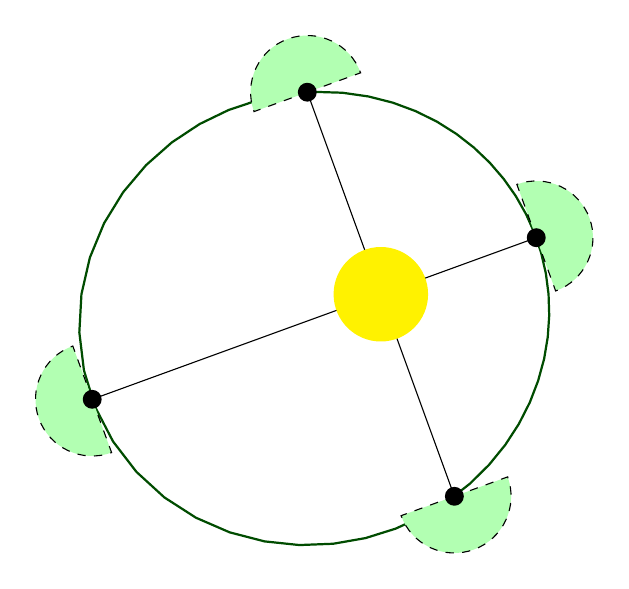
\begin{tikzpicture}[scale=1.2]

    \coordinate (S) at (0, 0);

    \pgfmathsetmacro{\e}{0.3} % set = keep float
    \pgfmathsetmacro{\p}{2.5}
    \pgfmathsetmacro{\aop}{20}

    % Orbits
    \foreach \s in {1,...,50}
        {
            \pgfmathsetmacro{\theta}{360/50*(\s-1)}  % define angle
            \draw (S) +(\theta:{\p*(1-\e^2)/(1 + \e*cos(\theta-\aop))}) coordinate (ORB1\s);
        }
    \draw[green!30!black, thick] (ORB11) foreach \s in {2,...,50}{-- (ORB1\s)} -- cycle;

    \pgfmathsetmacro{\arcsize}{0.6}

    \foreach \theta in {20, 110, 200, 290}
        {
            \pgfmathsetmacro{\radius}{\p*(1-\e^2)/(1 + \e*cos(\theta-\aop))}
            \draw (S) -- ++(\theta:\radius) coordinate (SC\theta);
            \filldraw[dashed, fill=green!30!white] (SC\theta) -- ++(\theta+90:\arcsize) arc(\theta+90:\theta-90:\arcsize) -- cycle;
            \fill[black] (SC\theta) circle (0.1cm);
        }

    \fill[yellow] (S) circle (0.5cm);

\end{tikzpicture}